\documentclass[11pt,a4paper]{article}

\usepackage[utf8]{inputenc}
\usepackage[english]{babel}
\usepackage[T1]{fontenc}

\usepackage{amsmath,amssymb,amsfonts}

\usepackage{tikz}
\usetikzlibrary{shapes,arrows}
\usepackage{tkz-graph}

\usepackage{graphicx}
\usepackage{hyperref}
\usepackage{mathtools}
%\mathtoolsset{showonlyrefs}

\title{Advanced Algorithms\\Assignment 2}
\author{Kristoffer Søholm \and Sebastian Tørholm \and Oskar Behrendt}

\begin{document}
\maketitle

\section{Exercise 1: Theory}
\subsection{Definition of $TCP$}
Let $G = (V, E)$ be a weighted graph with distance measure $d$,
$r \geq 0$ be the sight distance and $P$ be a cycle in $G$. We say
that $P$ is a \emph{sightseeing tour} if there for all $v \in V$ exists a
$w \in P$, such that $d(v, w) \leq r$. We then define the \emph{traveling
couple problem}, to be the problem of finding a sightseeing tour $T$ minimizing
the \emph{tour length}, $\sum_{(v,w) \in T} d(v, w)$.

We then define the related decision problem $TCP$ to be the problem of determining
whether there exists sightseeing tour of length at most $l$ in $G$. More formally,

\begin{align*}
    TCP = \{ \langle G, d, r, l \rangle :\ & G = (V,E) \text{ is a complete graph}, \\
                                           & d \text{ is a distance measure on } G, \\
                                           & r \geq 0, \\
                                           & G \text{ has a sightseeing tour with tour length at most } l \}
\end{align*}

\subsection{Reduction from $HAM-CYCLE$}
We wish to show that any instance of $HAM-CYCLE$ can be reduced to an instance of $TCP$.

Let $G = (V, E)$ be a graph, we then define $G'$ to be the complete graph with
the vertices $V$, and define a distance function $d$ on $G'$, given by
\[
    \forall v, w \in V : d(v, w) = \begin{cases} 1\ \ \text{if}\ \ e_{vw} \in E \\
                                                 2\ \ \text{otherwise}
                                   \end{cases} 
\]
Furthermore, let $r = \frac{1}{2}$.

We now claim, that any minimal solution to $TCP$ in $G'$ corresponds to
a Hamiltonian cycle in $G$.

Since the distance between any two vertices is greater than the sight radius,
we must have that all vertices are visited in order for $TCP$ to be solved.
Furthermore, we know that any sightseeing tour is a cycle by definition. Since a
Hamiltonian cycle makes use of precisely $|V|$ edges, and each edge has a weight of
at least $1$, we have that a any Hamiltonian cycle in $G'$ must have length at least $|V|$.

In particular we notice, that the length of the tour is $|V|$, and thus minimal,
whenever the tour is a Hamiltonian cycle in the original graph $G$.

This gives us, that
\[
    \langle G', d, r, |V| \rangle \in TCP \Rightarrow \langle G \rangle \in HAM-CYCLE,
\]
which provides the reduction that proves $TCP$ to be NP-complete.

\subsection{Exercise 1.2}
An obvious, if rather trivial, example is the following graph (borrowed from exercise 2).

\centerline{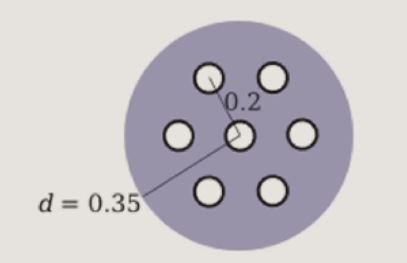
\includegraphics[width=0.4\textwidth]{tcp.png}}

Here the optimal TCP is simply to start at the middle vertex and stay there, which has a length of 0, which is shorter than any 1-tree.

\subsection{Exercise 1.3}
We have chosen to use the following ILP:

\label{ex13}
\begin{align}
    minimize & \sum_i \sum_j d(v_i, v_j) e_{ij} \nonumber \\
    s.t.     & \nonumber \\ 
             % each edge must be either used (1) or not used (0)
             & \forall i, j: e_{ij} \geq 0 \label{used} \\
             & \forall i, j: e_{ij} \leq 1 \label{used2} \\
             % 0 <= incoming + outgoing <= 2
             & \forall i: \sum_j (e_{ji} + e_{ij}) \leq 2 \label{nobranch} \\
             % incoming - outgoing = 0
             & \forall i: \sum_j (e_{ji} - e_{ij}) = 0 \label{nostop}\\
             % an edge can't be used in both directions
             & \forall i,j: e_{ji} + e_{ij} \leq 1 \label{nobidir} \\
             % w_i = exists(incoming)
             & \forall i: (\sum_j e_{ji}) - w_i = 0 \label{defw} \\
             % at least one vertex visited in the viscinity 
             & \forall i: \sum_{j \in v(i)} w_j \geq 1 \label{allseen}
\end{align}

Here we let $e_{ij}$ be $1$ if the edge $(i,j)$ is used in the path and $0$ otherwise.
Similarly $w_i$ denotes the use of vertex $i$.

\begin{itemize}
    \item \autoref{used} and \autoref{used2} ensures that every edge must either be used or unused.
    \item \autoref{nobranch} ensures that there are no branches in the path.
    \item \autoref{nostop} ensures that if a vertex is entered it is also exited from.
    \item \autoref{nobidir} ensures that each edge is used in only one direction in the path.
    \item \autoref{defw} sets $w_i$ to $1$ if vertex $i$ is visited or $0$ otherwise.
    \item \autoref{allseen} ensures that all vertices are seen during the tour.
\end{itemize}


\section{Exercise 2: Practice}

\subsection{Exercise 2.1}
We have implemented the lower-bound method using the ILP described in \autoref{ex13},
with no relaxed constraints.

The source code for the ILP lower bound solver can be found in \texttt{ILPLowerBound.java},
with each constraint described in its own method.

The implementation makes use of the Java wrapper to \texttt{lp\_solve}, which
can be found at \url{http://lpsolve.sourceforge.net/5.5/Java/README.html}.
Note, we did experience some bugs with the wrapper when trying to run it on a
64-bit machine. We would therefore advise to run it on a 32-bit machine instead.

\subsection{Exercise 2.2}
\begin{figure}[h!]
    \centering
    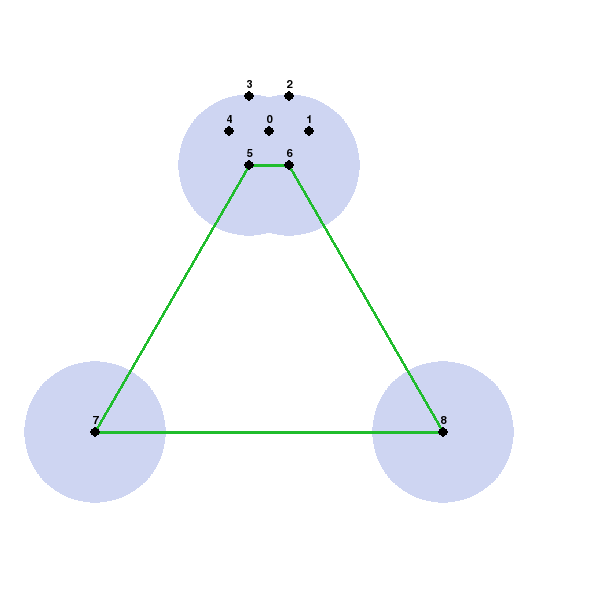
\includegraphics[width=0.4\textwidth, trim=0px 0px 200px 0px]{graph1.png}
    \caption{Graph1, tour length 4.9962, evaluated 76 nodes}
\end{figure}
\begin{figure}[h!]
    \centering
    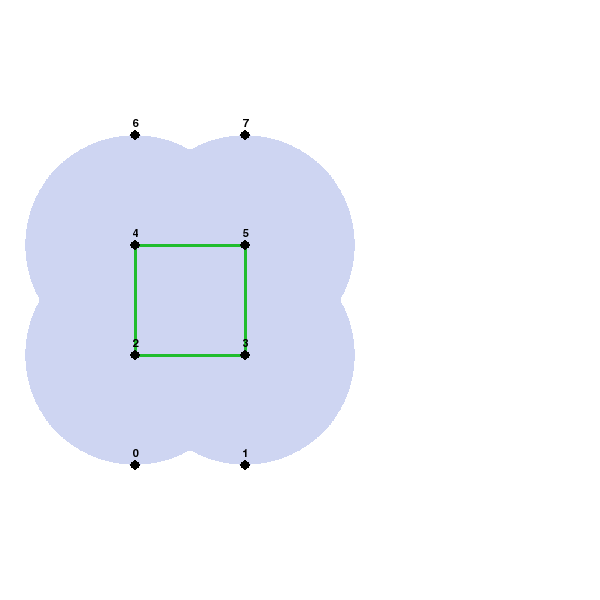
\includegraphics[width=0.4\textwidth, trim=0px 0px 200px 0px]{graph2.png}
    \caption{Graph2, tour length 4.0000, evaluated 32 nodes}
\end{figure}
\begin{figure}[h!]
    \centering
    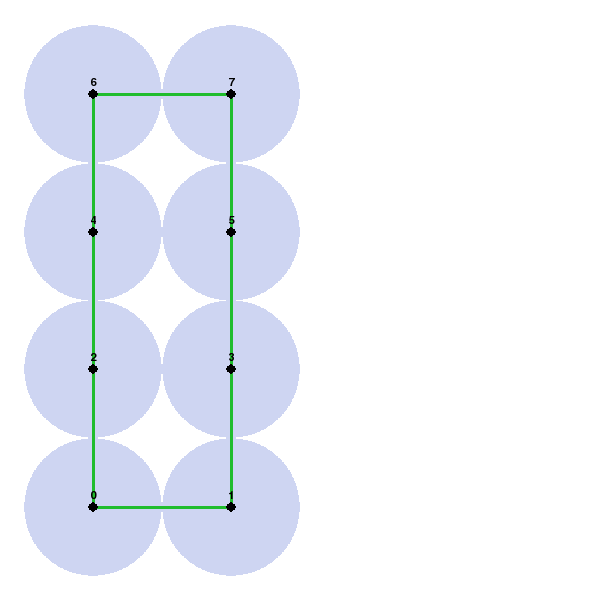
\includegraphics[width=0.4\textwidth, trim=0px 0px 300px 0px]{graph3.png}
    \caption{Graph3, tour length 8.0000, evaluated 55 nodes}
\end{figure}


\bibliographystyle{plain}
\bibliography{references.bib}
\end{document}
